\documentclass[12pt]{article}

\usepackage{fancyhdr}
\usepackage{amsthm}
\usepackage{amsmath}
\usepackage{graphicx}
\usepackage{amssymb}
\usepackage{esint}
\usepackage{subfigure}
\usepackage{color}
\usepackage{moreverb}

\textwidth 17cm \topmargin -1cm \oddsidemargin 0cm \textheight 21.5cm
\pagestyle{empty} \pagestyle{fancyplain}
\lhead[\fancyplain{}{}]{\fancyplain{}{{\sc Mario Infante}}}
\chead[\fancyplain{}{}]{\fancyplain{}{{\sc Collision Simulation}}}
\rhead[\fancyplain{}{}]{\fancyplain{}{{\sc Fall 2016}}}

\newcommand{\etal}{\textit{et al. }}

\begin{document}
\centerline{\Large\textbf{Simulation of Billiards}}
\vspace{2cm}


\section{Initial Movement}\label{sec::Intro}
\paragraph{•} 
For the initial movement of the disks the equation I used was the Euler Method equation. I took the initial position of the disk and added the product of my time step (dt) and the velocity to get its new positions. The new position would go through checks for various collisions before finally being drawn. This approach helped move the ball along the XY axis with X and Y velocities as shown in Figure 1. 

\section{Wall Collisions}
For detecting wall collisions, I used the distance formula to check whether the position with the radius of the disk was out of bounds. If so, I would reset the position of the disk to just touch the wall then multiply its x or y velocity by negative one depending on whether it hit a top/bottom or side wall.

\section{Disk Collisions}

For detecting disk collisions, I also used the distance formula but this time it was between both disks with their radii. I checked whether the position with the radius of the disks would overlap with each other and if so I would reset their positions so that they're just touching. Then I would multiply their velocities to a Normal and Tangential vector so that their velocities are reflected on a Normal/Tangential axis rather than XY axis. The normal velocities are swapped and then the vectors are multiplied by the inverse of Normal and Tangent vectors to revert back to the XY axis. The next positions are then updated and drawn. This process is shown in Figures 2 to 4.

\begin{figure}
\begin{center}
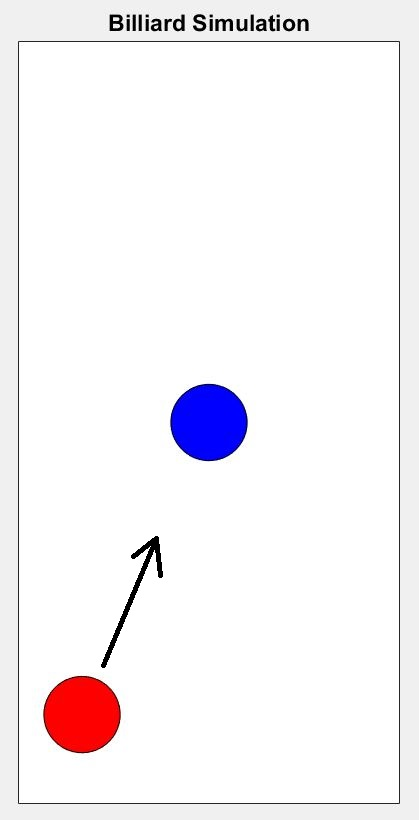
\includegraphics[width=.5\textwidth]{starting_position}
\end{center}
\caption{Disks in their starting positions.} \label{fig::MyFigure}
\end{figure}

\begin{figure}[h]
\begin{center}
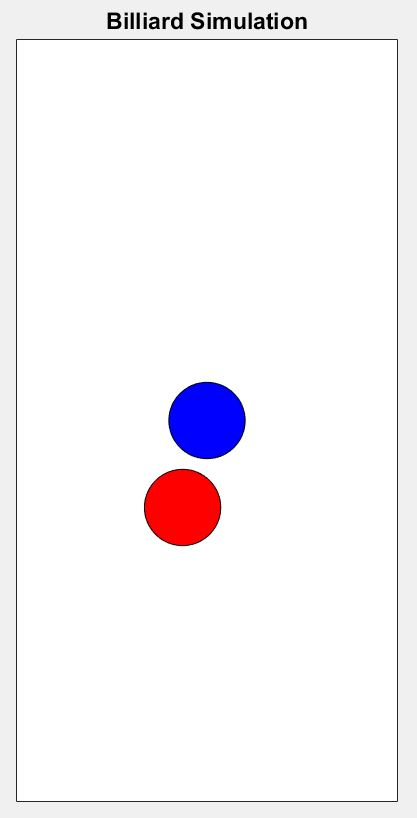
\includegraphics[width=.5\textwidth]{before_collision}
\end{center}
\caption{Disks right before collision.} \label{fig::MyFigure}
\end{figure}

\begin{figure}[h]
\begin{center}
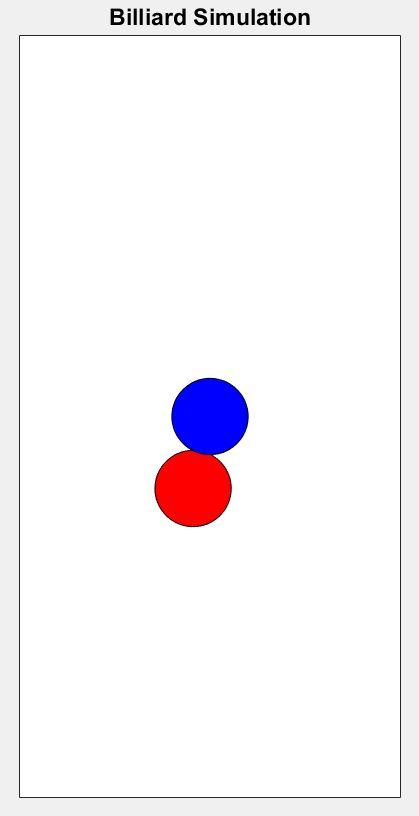
\includegraphics[width=.5\textwidth]{collision}
\end{center}
\caption{Disks at collision.} \label{fig::MyFigure}
\end{figure}

\begin{figure}[h]
\begin{center}
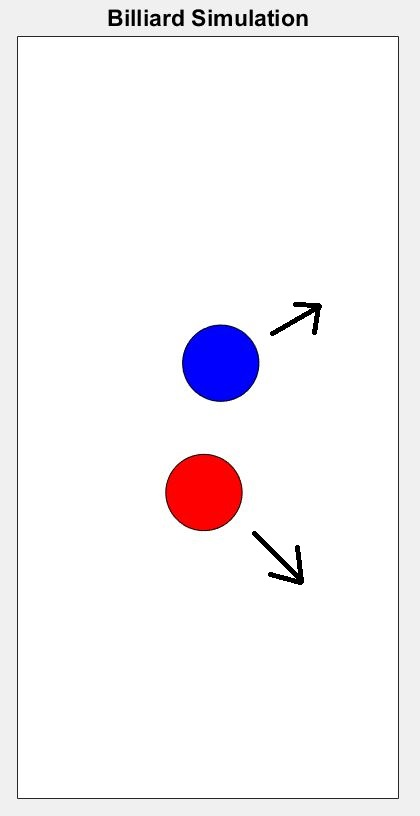
\includegraphics[width=.5\textwidth]{after_collision}
\end{center}
\caption{Disks after the collision.} \label{fig::MyFigure}
\end{figure}

\clearpage
\appendix
\section{Matlab Code}\label{sec::appendix}
The MATLAB code used for the Billiard Simulation is given below:
\begin{verbatimtab}

%BilliardSimulation.m
r = 0.1;            % radius
t = 0;
dt = 0.03;          % time step
a = 0.8;            % normal damping
b = 0.99;           % tangential damping
t_final = 5;

u1 = 2.24;
v1 = 4.48;
x1 = r;
y1 = r;
u2 = 0;
v2 = 0;
x2 = l/4;
y2 = l/2;
l = 2;


while t < t_final
    if t+dt > t_final
        dt = t_final - t;
    end
   
    
    % update positions
    x1 = x1 + dt*u1;
    y1 = y1 + dt*v1;
    x2 = x2 + dt*u2;
    y2 = y2 + dt*v2;    
    
    %left wall
    if(x1 + r >= l/2)
        u1 = a * -u1;
        v1 = b * v1;
        x1 = l/2 - r;
    end
    if(x2 + r >= l/2)
        u2 = a * -u2;
        v2 = b * v2;
        x2 = l/2 - r;
    end
    
    %right wall
    if(x1 - r <= 0)
        u1 = a * -u1;
        v1 = b * v1;
        x1 = r;
    end
    if(x2 - r <= 0)
        u2 = a * -u2;
        v2 = b * v2;
        x2 = r;
    end
    
    %bottom wall
    if(y1 + r >= l)
        v1 = a * -v1;
        u1 = b * u1;
        y1 = l - r;
    end
    if(y2 + r >= l)
        v2 = a * -v2;
        u2 = b * u2;
        y2 = l - r;
    end
    
    %top wall
    if(y1 - r <= 0)
        v1 = a * -v1;
        u1 = b * u1;
        y1 = r;
    end
    if(y2 - r <= 0)
        v2 = a * -v2;
        u2 = b * u2;
        y2 = r;
    end    
    
    %Detect Collision
    if(sqrt((x2 - x1)^2 + (y2 - y1)^2) - 2*r <= 0)
        tempdt = dt;
        dt = (sqrt((x2 - x1)^2 + (y2 - y1)^2) - 2*r)/sqrt((u2-u1)^2 + (v2-v1)^2);
        
        x2 = x2 + dt*u2;
        y2 = y2 + dt*v2;
        x1 = x1 + dt*u1;
        y1 = y1 + dt*v1;
        pause(.0001);
        Draw_Disks(l,x1,y1,x2,y2,r);
        
        angle=atan2(y2-y1,x2-x1);
        if abs(y2-y1)<1e-12
            if x2-x1>0
                angle = 0;
            else
                angle = pi;
            end
        end       

        N=[cos(angle) sin(angle)];
        T=[-sin(angle) cos(angle)];

        % Shifting coordinates from XY to Normal/Tangent with dot product
        vrnt = [u1*N(1)+v1*N(2) u1*T(1)+v1*T(2)];
        vbnt = [u2*N(1)+v2*N(2) u2*T(1)+v2*T(2)];
       
        
        %swap x velocities
        temp = vbnt(1);
        vbnt(1) = vrnt(1);
        vrnt(1) = temp;
        
        % Shifting coordinates back to XY and swapping x velocities
        % inverted dot products
        vrac = [vrnt(1)*T(2)+vrnt(2)*T(1) vrnt(1)*N(2) + vrnt(2)*N(1)];
        vbac = [vbnt(1)*T(2)+vbnt(2)*T(1) vbnt(1)*N(2) + vbnt(2)*N(1)];
        
        u1 = vrac(1);
        v1 = vrac(2);
        u2 = vbac(1);
        v2 = vbac(2);
        
        dt = tempdt;
        x2 = x2 + dt*u2;
        y2 = y2 + dt*v2;
        x1 = x1 + dt*u1;
        y1 = y1 + dt*v1;
        
    end
   
    pause(.001);
    Draw_Disks(l,x1,y1,x2,y2,r);
    t = t + dt;
end

%Draw_Disks.m
function outvar=Draw_Disks(l,x,y,a,b,r)
n=100;
for i=1:n
    theta=i*(2*pi/n);
    X(i)=x+r*cos(theta);
    Y(i)=y+r*sin(theta);
    A(i)=a+r*cos(theta);
    B(i)=b+r*sin(theta);
end
fill(X,Y,'r',A,B,'b'); % fills (in red 'r') the 2-D polygon defined by vectors X and Y
axis equal;
limits = [0 l/2 0 l];
axis (limits);
title('Billiard Simulation','FontSize',14);
set(gca,'xtick',[]); set(gca,'xticklabel',[]);
set(gca,'ytick',[]); set(gca,'yticklabel',[]);
end

\end{verbatimtab}

\end{document}
